g% --- Template for thesis / report with tktltiki2 class ---

\documentclass[finnish]{tktltiki2}

% tktltiki2 automatically loads babel, so you can simply
% give the language parameter (e.g. finnish, swedish, english, british) as
% a parameter for the class: \documentclass[finnish]{tktltiki2}.
% The information on title and abstract is generated automatically depending on
% the language, see below if you need to change any of these manually.
% 
% Class options:
% - grading                 -- Print labels for grading information on the front page.
% - disablelastpagecounter  -- Disables the automatic generation of page number information
%                              in the abstract. See also \numberofpagesinformation{} command below.
%
% The class also respects the following options of article class:
%   10pt, 11pt, 12pt, final, draft, oneside, twoside,
%   openright, openany, onecolumn, twocolumn, leqno, fleqn
%
% The default font size is 11pt. The paper size used is A4, other sizes are not supported.
%
% rubber: module pdftex

% --- General packages ---

\usepackage[utf8]{inputenc}
\usepackage{lmodern}
\usepackage{microtype}
\usepackage{amsfonts,amsmath,amssymb,amsthm,booktabs,color,enumitem,graphicx}
\usepackage[pdftex,hidelinks]{hyperref}

% Automatically set the PDF metadata fields
\makeatletter
\AtBeginDocument{\hypersetup{pdftitle = {\@title}, pdfauthor = {\@author}}}
\makeatother

% --- Language-related settings ---
%
% these should be modified according to your language

% babelbib for non-english bibliography using bibtex
\usepackage[fixlanguage]{babelbib}
\selectbiblanguage{finnish}

% add bibliography to the table of contents
\usepackage[nottoc,numbib]{tocbibind}
% tocbibind renames the bibliography, use the following to change it back
\settocbibname{Lähteet}

% --- Theorem environment definitions ---

\newtheorem{lau}{Lause}
\newtheorem{lem}[lau]{Lemma}
\newtheorem{kor}[lau]{Korollaari}

\theoremstyle{definition}
\newtheorem{maar}[lau]{Määritelmä}
\newtheorem{ong}{Ongelma}
\newtheorem{alg}[lau]{Algoritmi}
\newtheorem{esim}[lau]{Esimerkki}

\theoremstyle{remark}
\newtheorem*{huom}{Huomautus}


% --- tktltiki2 options ---
%
% The following commands define the information used to generate title and
% abstract pages. The following entries should be always specified:

\title{Ketterien menetelmien ratkaisuja ohjelmistotuotannon ja suunnitelmavetoisten menetelmien ongelmiin}
\author{Jarl-Erik Malmström}
\date{\today}
\level{Kandidaatintutkielma}
\abstract{Suunnitelmavetoiset menetelmät eivät sovi nopeasti muuttuvaan internet-aikakauden liiketoimintaympäristöön. Tarvitaan nopeasti reagoivia ja mukautuvia kehitysmenetelmiä. Ketterät menetelmät tarjoavat ratkaisuja muuttuviin vaatimuksiin ohjelmistokehityksen aikaisella kevyellä suunnitteluprosessilla. Ketterillä menetelmillä voidaan laatua unohtamatta toteuttaa käyttäjien toiveita vastaava ohjelmistojärjestelmä. Osa ketterien menetelmien käytänteistä parantaa ohjelmiston laatua ja ovat kustannustehokkaita kun otetaan huomioon laadunvarmistuksen kustannukset.}

% The following can be used to specify keywords and classification of the paper:

\keywords{agile, ketterä, iteraatiivinen, vesiputousmalli, spiraalimalli, pariohjelmointi, testivetoisuus}
\classification{Software development process management, Software development methods, Agile software development, Waterfall model, Spiral model} % classification according to ACM Computing Classification System (http://www.acm.org/about/class/)
                  % This is probably mostly relevant for computer scientists

% If the automatic page number counting is not working as desired in your case,
% uncomment the following to manually set the number of pages displayed in the abstract page:
%
% \numberofpagesinformation{16 sivua + 10 sivua liitteissä}
%
% If you are not a computer scientist, you will want to uncomment the following by hand and specify
% your department, faculty and subject by hand:
%
% \faculty{Matemaattis-luonnontieteellinen}
% \department{Tietojenkäsittelytieteen laitos}
% \subject{Tietojenkäsittelytiede}
%
% If you are not from the University of Helsinki, then you will most likely want to set these also:
%
% \university{Helsingin yliopisto}
% \universitylong{HELSINGIN YLIOPISTO --- HELSINGFORS UNIVERSITET --- UNIVERSITY OF HELSINKI} % displayed on the top of the abstract page
% \city{Helsinki}
%


\begin{document}

% --- Front matter ---
\pagestyle{empty}
\maketitle        % title page
\makeabstract     % abstract page

\tableofcontents  % table of contents
\newpage          % clear page after the table of contents


% --- Main matter ---

\pagestyle{plain}
\setcounter{page}{1}
\section{Johdanto}

Ohjelmistotuotannossa (software development) käytetään työn suunnitteluun ja organisointiin ohjelmistotuotantomenetelmiä (software development methodologies). Menetelmät määrittelevät muodollisen prosessin, jonka lopputuloksena syntyy ohjelmistojärjestelmä.

Ohjelmistotuotannon alkuaikoina tietokoneet olivat kookkaita sekä niiden käyttö\-kustannukset olivat ohjelmistoja tuottavien insinöörien palkkoihin verrattuna korkeat. Korkeista kustannuksista johtuen ohjelmistotuotannossa tarvittiin suunnittelua sekä järjestelmällisiä käytäntöjä. Tietojen\-käsittelyä ei tutkittu itsenäisenä tieteenalana, ja ohjelmistojen parissa työsken\-televät olivat muiden alojen insinöörejä sekä matemaatikkoja. Ohjelmistotuotannon menetelmät olivat omaksuttu muista insinööritieteistä \cite{BOE06}.

Ohjelmistojen merkityksen kasvaessa ihmisten ja tietokoneiden vuorovaikutus korostui yhä enemmän. Ohjelmistoalalle tarvittiin lisää ihmisiä tuottavaan ja luovaan työhön sekä enemmän insinöörejä ja matemaatikkoja kuin oli saatavilla. Ohjelmistotuotantoprojekteihin palkattiin muiden alojen asiantuntijoita, jotka omaksuivat helpommin \textit{ohjelmoi ja korjaa} (code and fix) lähestymistavan kuin insinöörien käytäntänteet \cite{BOE06}. Ohjelmoi ja korjaa menetelmällä kirjoitetaan ohjelmakoodia ilman perusteellista suunnittelua. Ohjelmistoa korjataan vikojen ilmaantuessa sekä ohjelmiston rakennetta, testausta ja ylläpitoa pohditaan myöhemmin \cite{BOE88}.

Eroavaisuudet perinteisten insinöörimenetelmien ja ohjelmoi ja korjaa asenteiden välillä loi uutta hakkerikulttuuria merkittävien yliopistojen tietojenkäsittelylaitoksille. Nämä auktoriteetteja vastustavat luovat sankariohjelmoijat tekivät ohjelmoi ja korjaa käytänteillä usein vaikeasti muutettavaa ja ylläpidettävää ohjelmakoodia \cite{BOE06}. Tällainen menetelmä saattoi toimia jos tuotettava ohjelmisto on pieni, mutta järjestelmän kasvaessa uusien toiminnallisuuksien lisääminen vaikeutui. Lisäksi virheiden löytäminen ja korjaaminen vaikeutui järjestelmän kasvaessa \cite{FOW01a}.

Ohjelmistotuotannon parissa työskentelevät huomasivat, että ohjelmiston kehitykseen liittyvät ilmiöt poikkesivat huomattavasti laitteistoihin liittyvistä ilmiöistä. Laitteistoille laadituilla luotettavuusmalleilla ei voitu arvioida ohjelmistojen luotettavuutta kattavasti. Ohjelmistoprojektien aikatauluja oli vaikea ennakoida, ja henkilöstön lisääminen aikataulun nopeuttamiseksi saattoi myöhästyttää projektia entisestään \cite{BOE06}.

Ohjelmistotuotantoon tarvittiin paremmin organisoituja menetelmiä ja kurinalaisia käytäntöjä yhä suurempien projektien hallinointiin. Reaktiona ohjelmoi ja korjaa menetelmille kehitettiin uusia prosessimalleja, joilla pyrittiin parantamaan 1950-luvun insinöörimenetelmien käytänteitä ohjelmistotuotantoon liittyvillä tekniikoilla. Näissä prosessimalleissa ohjelmointia edelsi kattava suunnittelu-, määrittely-, ja analysointivaihe. Näitä menetelmiä kutsutaan suunnitelmavetoisiksi (plan-driven) \cite{BOE02} tai dokumenttivetoisiksi (document-driven) \cite{BOE88} menetelmiksi. Tässä tutkielmassa käytämme näistä yhteisesti käsitettä suunnitelmavetoinen menetelmä.

Internetin laajentuminen ja \textit{hypertekstijärjestelmän} (World Wide Web) ilmaantuminen korostivat ohjelmistojen merkitystä. Ohjelmistojen merkitys yritysten kilpailutekijänä ja liiketoimintaympäristön jatkuvat ja muutokset lisäsivät tarvetta lyhentää ohjelmistotuotantoon kuluvaa aikaa. Suunnittelua, määrittelyä ja dokumentointia painottavat menetelmät eivät sopineet jatkuvasti muuttuvaan liiketoimintaympäristöön ja nopeaan ohjelmistokehitykseen (rapid application development)\cite{BOE06}.

Tässä tutkielmassa tarkastelemme myös ketteriä menetelmiä (agile methods). Suunnitelmavetoiset menetelmät ovat saaneet kritiikkiä osakseen ja ketterät menetelmät ovat olleet reaktio suunnitelmavetoisten menetelmien heikkouksille sopeutua muutoksiin. Ketterät menetelmät pyrkivät kompromissiin, ohjelmoi ja korjaa-menetelmän ja suunnitelmavetoisen menetelmän väliltä, tarjoamalla riittävän prosessin haluttuun lopputulokseen pääsemiseksi \cite{FOW01a}. 

Käymme läpi erilaisia suunnitelmavetoisia ja ketteriä menetelmiä sekä näiden lähestymistapoja ohjelmistotuotantoon. Selvitämme ohjelmiston laatuun liittyviä käsitteitä ja tarkastelemme ohjelmistotuotannon haasteita. Esittelemme, miten ketterät menetelmät ratkaisevat esitettyjä ohjelmistotuotannon haasteita ja tarkastelemme onko ketterien menetelmien käytänteillä vaikutusta ohjelmistojen laatuun.

Tutkielman rakenne on seuraava: Kappaleessa kaksi käsittelemme ohjelmistotuotannon haasteita ja laatuun liittyviä käsitteitä. Kappaleessa kolme käymme läpi erilaisia suunnitelmavetoisia ja ketteriä menetelmiä. Kappaleessa neljä selvitämme ketterien menetelmien ratkaisuja suunnitelmavetoisten menetel\-mien ongelmiin ja ohjelmistotuotannon haasteisiin. 

\section{Ohjelmistotuotannon haasteet ja ohjelmistojen laatu}

Tässä kappaleessa käymme läpi erilaisia ongelmia ja haasteita, joita ohjelmistotuotantoprojekteissa usein ilmenee. Esille tuomamme ohjelmistotuotannon haasteet liittyvät erityisesti suunnitelmavetoisten menetelmien käytänteisiin. Tämän jälkeen selvitämme ohjelmistojen laatuun liittyviä määritelmiä sekä miten ohjelmistotuotannossa ilmenevät ongelmat liittyvät ohjelmistojen laatuun.

Ohjelmistotuotantoprojekteissa usein ilmenee monia haasteita projektin koordinointiin sekä valmiin ohjelmiston toimintaan liittyen. Ohjelmistotuotannossa ilmenevät haasteet voidaan jakaa seuraaviin osa-alueisiin: henkilöstön hallinta, projektin aikataulu ja taloudelliset resurssit, vaatimusten hallinta, tekniset valmiudet ja projektin mahdolliseen ulkoistukseen liittyvät ongelmat \cite{BOE88}.

Suunnitelmavetoisissa menetelmissä asiakas on ohjelmistoprojektissa tiiviissä yhteistyössä kehittäjäorganisaation kanssa usein vain ohjelmistoa suunniteltaessa. Ohjelmistoa rakennettaessa asiakasyhteistyö on usein vähäistä itse kehittäjätiimin kanssa. Vähäinen asiakasyhteistyö voi johtaa erilaisiin ongelmiin: Ohjelmistoon saatetaan kehittää toiminnallisuuksia, joita ei tarvita tai ne ovat väärin määriteltyjä. Käyttöliittymästä voi olla vaikeakäyttöinen tai puutteellinen. Koska ohjelmoijat eivät ole tiiviissä yhteistyössä asiakkaan kanssa, tarvittavien toiminnallisuuksien yksityiskohdat saattavat jäädä epäselviksi. Jos asiakas ei ole kehittäjätiimin saatavilla, ohjelmoijat joutuvat tekemään ratkaisuja puutteellisten tietojen varassa  \cite{BOE88}.

Vaadittavien toiminnallisuuksien epäselvyydestä ja ohjelmoijien omasta ammatillisesta kiinnostuksesta johtuen, ohjelmoijat voivat lisätä tarpeettomia toiminnallisuuksia. Väärien ja tarpeettomien toiminnallisuuksien kehitys ohjelmistotuotantoprojektin resursseja ja nostaa ohjelmistokehitykseen vaadittavia kustannuksia. \cite{BOE88}.

Suunnitelmavetoisissa menetelmissä ohjelmistojärjestelmän suunnitelmat on saatava valmiiksi ennen kuin sitä voidaan alkaa rakentamaan. Ohjelmiston kattava suunnittelu ennen sen rakentamista on kuitenkin vaikeaa, koska on vaikea huomioida kaikkia yksityiskohtia ohjelmiston toimintaympäristöön ja operatiiviseen toimintaan liittyen \cite{BOE88}.

Puutteellisista tiedoista johtuen ohjelmistot eivät usein tyydytä käyttäjien tarpeita. Ohjelmistotuotannon kehitys pitkittyy, kun ohjelmistoa on muutettava käyttäjien tarpeita vastaavaksi. Ohjelmistotuotantoon varattu aikataulu ja budjetti kasvaa, kun ohjelmistojärjestelmää pitää uudelleen suunnitella ja rakentaa \cite{BEC99}.

Suunnitelmavetoisissa menetelmissä ohjelmistojärjestelmän oikeanlainen ja haluttu toiminta on varmistettu ohjelmistokehityksen loppuvaiheessa tehtävällä ohjelmistotestauksella: kirjoitettu ohjelmakoodi varmistetaan testaavalla koodilla, joka käy läpi ohjelmiston eri vaiheita, erilaisilla syötteillä sekä tulostuksilla. Tuloksilla voidaan päätellä toimiiko rakennettu järjestelmä oikein. Ohjelmistokehitysjakson lopussa vasta testausvaiheessa voi ilmetä ongelmia, joihin analyysilla ja suunnittelulla ei ole voitu varautua. Testauksessa ilmenevät ongelmat saattavat johtaa muutoksiin järjestelmän vaatimusmäärittelyssä ja ohjelmiston suunnittelussa. Lisääntynyt suunnittelu- ja määrittelytyö johtavat jälleen kohoaviin ohjelmistotuotannon kustannuksiin \cite{ROY70}.

Ohjelmistotestauksessa saattaa ilmetä myös rakennetun järjestelmän odotettua heikompi suorituskyky. Toisaalta tietotekniset mahdollisuudet on voitu arvioida väärin eikä käytössä olevien tietokoneiden laskentakyky riitä suunniteltuun järjestelmään \cite{BOE88}.
 
\subsection{Koordinointi}

Tässä tutkielmassa koordinoinnilla tarkoitamme yksilöiden ja ryhmien välistä yhteistoimintaa sekä näihin liittyvää hallinnollista työtä ja toisaalta ohjelmistojärjestelmän eri osien yhteensovittamista. Ohjelmistoprojektin koordinointiongelmat liittyvät henkilöstön, vaatimusten hallintaan \cite{KES95}.

Yksittäinen henkilö tai pieni ryhmä voi tehokkaasti koordinoida pienen ohjelmistojärjestelmän kehitystä ja hallinoida toteutuksen yksityiskohtia. Yksilöiden tai ryhmän on mahdotonta toteuttaa ja hallinnoida suuria, miljoonien rivien ohjelmakoodien, ohjelmistoja ja useiden vuosien ohjelmistokehitystä yksityiskohtaisesti \cite{KES95}.

Suuriin ohjelmistoprojekteihin saattaa liittyä useita kehittäjä\-organisaatioita ohjelmiston tilaajan lisäksi ja nämä onnistuvat useimmin jos projektia koordinoi henkilö, jolla on tietoa ohjelmiston kohdealueelta sekä ohjelmistoalalta. Kohdealueen tieto ei ole usein käytössä kaikilla projektiin osallistuvilla, koska suuret projektit johtavat työn erikoistumiseen ja jakamiseen. Organisaatiossa työn eriytyminen johtaa toisistaan riippuvien tekijöiden jakamiseen osastoihin maantieteellisesti, organisatorisesti, sekä sosiaalisesti. Tämä vähentää mahdollisuuksia ja haluja oppia sekä jakaa tietoa etäisten työtovereiden kesken ja kohdealueen tietoa katoaa \cite{KES95}.

Koordinointiongelma liittyy myös rakennettavaan ohjelmistojärjestelmään: ohjelmistot ovat pääasiallisesti rakennettu useista osista, jotka on kytkettävä yhteen ja ohjelmistojärjestelmän osien on toimittava koordinoidusti. Ohjelmistojen suuri koko aiheuttaa ongelmia, koska ohjelmisto vaatii sen osajärjestelmien täsmällistä integraatiota, jotta ohjelmisto toimisi oikein  \cite{KES95}.

Tiedon koordinointi eri organisaatioiden välillä on usein haasteellista. Ohjelmistokehityksessä haaste on, että ohjelmistoarkkitehtien ja -suunnittelijoiden sekä ohjelmoijien päätöksentekoon tarvitsema tieto ei ole saatavilla. Ohjelmiston toimintaan liittyvät tiedot usein muuttuvat ohjelmistoprojektin edetessä. Muutoksia ohjelmiston vaatimuksiin esiintyy, koska liiketoiminta, käyttäjien toiveet, tietokoneympäristö, ohjelmiston syötteet ja fyysinen maailma muuttuvat   \cite{KES95}.

\subsection{Suunnittelu ja muuttuvat vaatimukset}

Asiakkaalla on vaatimuksia kehitettävän järjestelmän toiminnallisuuksista, joita ohjelmoijat toteuttavat. Vaikeuksia ilmenee näiden vaatimuksien ymmärtämisessä ja usein vaatimukset muuttuvat projektin edetessä. Vaatimukset muuttuvat koska liiketoimintaympäristöt muuttuvat tai asiakkaat saattavat keksiä uusia toiminnallisuuksia toteutettavalle järjestelmälle \cite{FOW01a}.

Ohjelmistotuotannossa asiakkaiden vaatimien toiminnallisuuksien suunnittelu ja toteutus on haasteellista: tyypillisesti suunnitelmavetoisissa menetelmissä ohjelmistotuotantoprojektiin osallistuva henkilö vaihtelevalla kohdealueen tuntemuksella haastattelee asiakkaita ja käyttäjiä. Tämän jälkeen haastattelija kirjaa asiakkaan haluamat toiminnallisuudet ohjelmistoarkkitehdeille ja -suunnittelijoille. Merkityksellistä kohdealueen tietoa katoaa usein, koska asiakas ei osaa tuoda esille kaikkia tarpeitaan ja jotkin ilmoitetut tarpeet jäävät kirjaamatta.

Teknologian ja liiketoiminnan vaatimusten muuttuessa suunnitelmat vanhentuvat nopeasti \cite{WIC03}. Alkuperäisen suunnitelman seuraaminen ei ole ohjelmistoprojektien päämäärä, sen sijaan toimitettavan ohjelmiston tarkoitus on asiakkaan mahdollisesti muuttuvien tarpeiden tyydyttäminen \cite{HIC01}. Internet liiketoimintaympäristönä vahvistaa ohjelmistotuotannon ongelmia korostamalla nopeutta. Asiakkailla on epätoivoinen kiire markkinoille. He vaativat liiketoiminnalle arvoa tuottavia ominaisuuksia yhä nopeammassa tahdissa. \cite{BRL03}.

Muutostarpeita ilmestyy todennäköisemmin, kun käyttäjät käyttävät toimivaa ohjelmistoa. Tällöin käyttäjät näkevät ohjelmiston rajoitteet ja mahdollisuudet. Kun ihmiset käyttävät ohjelmistoa, niin he todennäköisesti keksivät uusia toiminnallisuuksia olemassa olevalle järjestelmälle \cite{KES95}. Ohjelmiston toiminnallisuuksien arvoja on vaikea nähdä ennen kuin ohjelmistoa käytetään oikeassa toimintaympäristössä \cite{FOW01a}.

Muuttuvat tai puutteelliset vaatimukset voidaan nähdä johtuvan heikosta suunnittelusta. Suunnitelmavetoisissa menetelmissä ajatuksena usein on saada selkeä kokonaiskuva toteutettavista toiminnallisuuksista ennen ohjelmiston rakentamista sekä rajoittaa asiakkaan vaatimia muutoksia asiakkaan ja kehittäjäorganisaation välisellä sopimuksella \cite{FOW01a}.

Ohjelmistojärjestelmältä vaadittavien toiminnallisuuksien hallinnointi on asiakkaan kannalta ongelmallista: erilaisten vaihtoehtojen vertailu on vaikeaa, koska ohjelmistokehittäjät eivät yleensä tarjoa hinta-arvioita erilaisista toiminnallisuuksista. Ilman tietoa hinnasta on vaikea arvioida halutaanko tietystä toiminnallisuudesta maksaa vai ei. Arviointi on vaikeaa, koska ohjelmistokehitys on suunnittelutyötä. \cite{FOW01a}. Toisin kuin teollinen valmistus, ohjelmistokehitys ei ole rutiininomainen toimi: ohjelmistoprojektit ovat yksilöllisiä eikä ohjelmistojärjestelmille usein ole valmiita prototyyppejä \cite{KES95}.

\subsection{Tekninen kehitys ratkaisuna}

Teknologian ja ohjelmistotuotantomenetelmien kehityksestä huolimatta, suuriin ohjelmistotuotantoprojekteihin liittyviä ongelmia ei ole onnistuttu lopullisesti ratkaisemaan.
Voidaan sanoa, että aikaisemmat korjaustoimenpiteet ovat lähestyneet ongelmia seuraavasti:
\begin{itemize}
\item Kehittämällä ohjelmistotuotannossa tarvittavia teknisiä työkaluja.
\item Jakamalla ohjelmisto osiin (modularization) teknisesti, esimerkiksi olio-ohjelmoinnilla (object-oriented programming).
\item Jakamalla ohjelmistotuotantoa hallinnollisesti: eriyttämällä vaatimus\-määrittelyn, ohjelmoinnin ja testaustoiminnot.
\item Formalisoimalla teknisiä menettelytapoja, esimerkiksi versionhallinta, testisuunnitelma ja vaatimusmäärittelydokumentit \cite{KES95}.
\end{itemize}

Nykyään ohjelmistokehittäjät käyttävät laajasti työkaluja, jotka nopeuttavat suunnittelu- ja ohjelmointiprosessia. Uuden teknologian työkalut tarjoavat toimintoja, jotka ennen oli toimitettava itse. Erilaiset ohjelmistokehykset (frameworks) tekevät osan ohjelmiston kehitystä. Ohjelmistokehitystä voidaan nopeuttaa komponenttien uudelleen\-käytöllä. Sen sijaan, että rakennettaisiin ohjelmisto alusta alkaen itse, valmiita komponentteja hankintaan, yhdistetään ja kootaan nopeasti \cite{BRL03}.

Nykyiset ohjelmistotyökalut eivät ole tarjonneet yksiselitteisiä ratkaisuja haasteisiin. Työkalut lisäävät yksilöiden tuottavuutta, mutta eivät ratkaise ohjelmistotuotannon koordinointiongelmaa. Onnistunut ohjelmistotuotantoprojekti vaatii lisäksi erilaisten näkemysten sekä ohjelmistojärjestelmän osien yhteensovittamista \cite{KES95}.

\subsection{Ohjelmistojen laatu}

Laatu on monitahoinen käsite ja sitä voidaan kuvailla viidestä eri näkökulmasta: \textit{Täydellisen näkemyksen} (transcendental view) mukaan laatua voidaan kuvailla, mutta ei määritellä eikä täysin toteuttaa. Täydellinen näkemys kuvaa ohjelmiston laatua ihanteena (ideal), mihin ohjelmiston toteutuksessa pyritään \cite{KIP96}. 

\textit{ Käyttäjänäkemys} (user view) laadusta liittyy konkreettisesti tuotteeseen, joka tyydyttää käyttäjän tarpeet. Käytettävyys on esimerkiksi sellainen tuotteen piirre, mikä liittyy käyttäjän näkemykseen laadusta. Käytettävyydellä tarkoitamme ohjelmiston käytöstä aiheutuvan todellisen ja oletetun vaivannäön suhdetta \cite{KIP96}.  

\textit{Tuotantonäkemys} (manufacturing view) tarkastelee laatua valmistusprosessien näkökulmasta. Näkemys liittyy tuotteen oikeanlaiseen valmistukseen ja ajatuksena on vähentää tuotteeseen tehtävistä muutoksista aiheutuvia kustannuksia \cite{KIP96}. 

 \textit {Tuotenäkemys} (product view) tarkastelee tuotteen sisäisiä ominaisuuksia ja näiden vaikutusta sisäiseen laatuun (internal quality). Tätä lähestymistapaa puolletaan usein oletuksella, että sisäistä laatua mittaamalla ja valvomalla parannetaan käyttäjän näkemykseen liittyvää tuotteen ulkoista laatua (external quality) \cite{KIP96}.  

 \textit{Arvovetoinen näkemys} (value-based view) tarkastelee laatua suhteessa siitä aiheutuviin kustannuksiin. Joskus edellä mainitut näkemykset voivat olla keskenään ristiriitaisia. Esimerkiksi jos käyttäjä haluaa uusia toiminnallisuuksia tai muutoksia ohjelmistoon ja toisaalta tuotantonäkemys pyrkii vähentämään muutoksia. Arvovetoinen näkemys auttaa löytämään tasapainon kustannusten ja laadun väliltä \cite{KIP96}.

Oletetaan, että tilattu ohjelmistojärjestelmä toimitetaan ajallaan ilman budjettia ylittäviä kustannuksia, ja se toimii oikein sekä suorittaa tehokkaasti sille määritetyt toiminnallisuudet. Voidaanko tuotteeseen tällöin olla tyytyväisiä? Ei välttämättä kaikissa tapauksissa. Ohjelmistojärjestelmää voi olla vaikea ymmärtää ja muuttaa. Ohjelmistoa ei välttämättä ole helppokäyttöinen. Ohjelmisto voi olla tarpeettoman laitteistoriippuvainen. Nämä seikat johtavat kohtuuttomiin ylläpitokustannuksiin \cite{BBL76}.
Kansainvälinen standardointiorganisaatio (ISO) on suositellut laadun perustaksi seuraavia itsenäisiä piirteitä: \cite{KIP96}

\begin{enumerate}
\item toiminnallisuus (functionality)
\item luotettavuus (reliability)
\item käytettävyys (usability)
\item tehokkuus (efficiency)
\item ylläpidettävyys (maintainability)
\item siirrettävyys (portabilty)
\end{enumerate}

Toiminnallisuudella ja luotettavuudella tarkoitamme seuraavaa: toiminnallisuuksien on tyydytettävä käyttäjän vaatimukset sekä kyettävä ylläpitämään vaadittu suorituskyky vaaditun ajan \cite{KIP96}.

Käytettävyys mittaa ohjelmistojärjestelmän käytöstä aiheutuvan ja käyttäjien olettaman vaivannäön suhdetta \cite{KIP96}. 

Tehokkuudella tarkoitamme suorituskyvyn sekä käytettyjen resurssien suhdetta ja yllä\-pidettävyydellä ohjelmistoon tehtäviin muutoksiin tarvittavaa työmäärää, jotka voivat liittyä korjauksiin, parannuksiin tai ohjelmiston mukauttamista muuttuneisiin olosuhteisiin \cite{KIP96}. 

Siirrettävyys viittaa ohjelmiston kykyyn toimia erilaisessa ympäristössä: toisessa organisaatiossa, laitteistossa tai ohjelmistoympäristössä \cite{KIP96}.

Yllä mainitut kansainvälisen standardointiorganisaation laatumallin piirteistä liittyvät käyttäjän näkemykseen (user view) ohjelmistosta ja miten se tyydyttää hänen tarpeensa. Tuotettavan ohjelmistojärjestelmän vaatimuksia edustaa käyttäjän tai asiakkaan tarpeet ja näkemys. Toimme esille, ohjelmistotuotannon haasteita käsitellessämme, asiakkaiden tarpeiden ja vaatimusten hallinnan aikaisemmin kappaleessa 2.2. Voimme todeta ohjelmistotuotannon haasteiden ja ohjelmiston laadun liittyvän toisiinsa sekä vaatimusten hallinnan liittyvän myös ohjelmiston laadun hallintaan \cite{KIP96}.

Seuraavaksi tarkastelemme suunnitelmavetoisia ja ketteriä menetelmiä sekä näiden käytänteitä. Myöhemmin käymme läpi ketterien menetelmien ratkaisuja ohjelmistotuotannon sekä suunnitelmavetoisten menetelmien haasteisiin.

\section{Suunnitelmavetoiset ja ketterät menetelmät}

Suunnitelmavetoiset ohjelmistotuotantomenetelmät ovat ohjelmistokehityksen yksityiskohtaisia ja kurinalaisia prosesseja, joiden tarkoituksena on tehdä ohjelmistotuotannosta ennustettavaa ja tehokasta sekä välttää ohjelmistotuotantoon liittyviä riskejä. Muista insinööritieteistä vaikutteita saaneet menetelmät ovat yksityiskohtaisia prosesseja, joissa painotetaan ennen ohjelmiston rakentamista tehtävää suunnittelutyötä \cite{FOW01a}.

Suunnitelmavetoisten menetelmien lähestymistapa perustuu oletukselle, että aikaisella ja täydellisellä vaatimusmäärittelyllä voidaan vähentää kehityksen aikana tulevia muutoksia ja niistä aiheutuvia kustannuksia. Ketterien menetelmien näkökulmasta muutosten kieltäminen merkitsee reagoimattomuutta liiketoimintaympäristön kehitykselle \cite{HIC01}.

Ketterissä menetelmissä kehittäjäorganisaatiot ovat valmiimpia reagoimaan muutoksiin ohjelmistokehityksen aikana kuin suunnitelmavetoisissa menetelmissä: kaikki kehityksen aikana esille tulleet uudet vaatimukset tai muutoksia kaipaavat valmiit toiminnallisuudet otetaan esille asiakkaan toimesta, ja ohjelmistoa kehitetään jatkuvasti yhteistyössä hänen kanssa \cite{WIC03}.

Käymme seuraavaksi läpi lyhyesti vesiputousmallin (waterfall model) ja spiraalimallin (spiral model) sekä näihin prosessimalleihin liittyviä ongelmia. Myöhemmin tarkastelemme miten ketterät menetelmät ovat pyrkineet ratkaisemaan näissä prosessimalleissa ilmenneitä ongelmia ja ohjelmistotuotannon haasteita.

\subsection{Vesiputousmalli}

Vesiputousmalli (waterfall model) on lineaarinen (kuvassa 1.) vaiheesta seuraavaan etenevä prosessimalli.1970-luvulla vesiputousmalli vaikutti suuresti lineaarisiin ohjelmistotuotannon suunnitelmavetoisiin prosessimalleihin. Vesiputousmallin lähestymistapa auttoi poistamaan monia aiemmin ohjelmistotuotantoa vaivanneita ongelmia: ohjelmoi ja korjaa mallilla ohjelmakoodista tuli korjausvaiheiden jälkeen usein kallista muuttaa, koska ohjelmakoodi oli rakenteellisesti huonoa eikä muutoksiin ja testaamiseen oltu varauduttu. Ohjelmoi ja korjaa mallilla tehdyt ohjelmistojärjestelmät eivät usein täyttäneet käyttäjien tarpeita, koska ne olivat rakennettu ilman tarkempaa suunnitelmaa ja analyysia \cite{BOE88}.

\begin{figure}[h!]
\caption{Lineaarinen ohjelmistotuotantoprosessi}
\centering
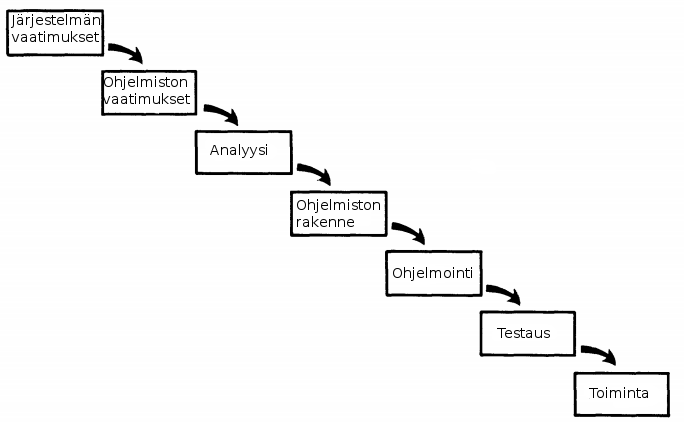
\includegraphics[width=\textwidth]{waterfall}
\end{figure}

Vesiputousmallissa ohjelmistotuotanto koostuu seuraavista vaiheista: järjestelmän ja ohjelmiston vaatimusmäärittely sekä analyysi, ohjelmistonrakenteen suunnittelu, ohjelmointi, testaus ja ohjelmiston käyttö \cite{ROY70}.

Määrittely- ja analyysivaiheessa kerätään kehitettävän järjestelmän ja ohjelmiston vaatimukset ja rajoitteet. Vaatimukset ovat joukko toiminnallisuuksia, joita loppukäyttäjä odottaa ohjelmistolta. Loppukäyttäjien vaatimuksien ja liiketoimintaympäristön analysointi on edellytys ohjelmiston rakenteen suunnittelulle. \cite{ROY70}.

Määrittely- ja suunnitteluvaiheen jälkeen suunnitellaan järjestelmän rakenne: ohjelmiston arkkitehtuuri, tarvittavat luokat ja niiden toiminnallisuus sekä komponenttien yhteensopivuus ja yhteistoiminta \cite{ROY70}.

Ohjelmointivaiheessa kirjoitetaan ohjelmakoodi laadittujen suunnitelmien perusteella ja testausvaiheessa ohjelmistojärjestelmän oikeanlainen toiminta varmistetaan etsimällä selviä virheitä tuotantokoodista visuaalisesti tarkastelemalla ja kirjoittamalla testitapauksia tuotantokoodin osille. Testitapaukset testaavat järjestelmän osia erilaisilla syötteillä sekä tarkastavat, että tulosteet ja järjestelmän tila ovat oikein  \cite{ROY70}.

Vesiputousmallissa painotetaan dokumentin tärkeyttä: Hyvän dokumentoinnin todellinen arvo ilmenee testausvaiheessa, ohjelmistoa käytettäessä sekä uudelleen suunniteltaessa. Hyvän dokumentin avulla esimies voi keskittää henkilöstön ohjelmistossa ilmenneisiin virheisiin. Ilman hyvää dokumenttia, ainoastaan ohjelmistovirheen alkuperäinen tekijä kykenee analysoimaan kyseessä olevan virheen. Dokumentin avulla ohjelmistojärjestelmää testaava henkilö voi ymmärtää järjestelmän toimintaa paremmin. Käyttöönotossa ilmenneiden ohjelmistovirheiden korjaamisessa selkeä dokumentti on välttä\-mätön \cite{ROY70}.

Vesiputousmallin ongelmana on dokumentaation korostuminen valmistumiskriteerinä aikaisille vaatimuksille ja suunnitteluvaiheille. Menetelmä ei sovi erityisesti interaktiivisiin loppukäyttäjien sovelluksiin, koska käyttäjät näkevät toimivaa ohjelmistoa ohjelmistotuotantoprojektin loppuvaiheessa. Dokumenttivetoisuus pakottaa kirjaamaan käyttö\-liittymien vaatimukset yksityiskohtaisesti, mutta käyttäjät eivät kykene tyhjentävästi kertomaan mitä toiminnallisuuksia ohjelmistolta haluavat. Asiakas saattaa muuttaa mielensä. Tai hän osaa usein sanoa, nähdessään valmiin tuotteen, mitä olisi ohjelmistolta halunnut \cite{BEC99}.

Muuttuvista vaatimuksista seuraa käyttökelvottoman ohjelmakoodin suunnittelua ja toteutusta. Muutosten kustannukset kasvavat ohjelmiston elinkaaren aikana: mitä pidemmälle projekti etenee sitä kalliimpaa muutosten tekeminen on \cite{HIC01}. Lineaarisen ohjelmistotuotantomenetelmän vaiheet ovat tällaisille projekteille selvästi väärässä järjestyksessä. Joillekin ohjelmistoille ei ole tarvetta yksityiskohtaiselle dokumentaatiolle ennen toteutusta \cite{BOE88}.


\subsection{Spiraalimalli}

Spiraalimallin (spiral model) tarkoitus oli edistää ohjelmistotuotantoprosessia lähestymällä ohjelmistoa iteratiivisesti (iterative) ja inkrementaalisesti (incremental) analysoimalla tuotannossa kohdattavia ongelmia. Tämä mahdollistaa mallin mukautumaan, kohdattavien riskien mukaan, painottamalla määrittelyä (specification), prototyyppien valmistusta, simulointia tai muita lähestymistapoja ohjelmiston suunnitteluun. Spiraalimalli on kehitetty vesiputousmallista saatujen kokemuksien perusteella \cite{BOE88}.
 
Kuvassa 2. oleva spriraalimallin jokainen vaihe pitää sisällään samat toimenpiteet: cite{BOE88}.

\begin{figure}[h!]

\caption{Spiraalimallin ohjelmiston elinkaari}
\centering
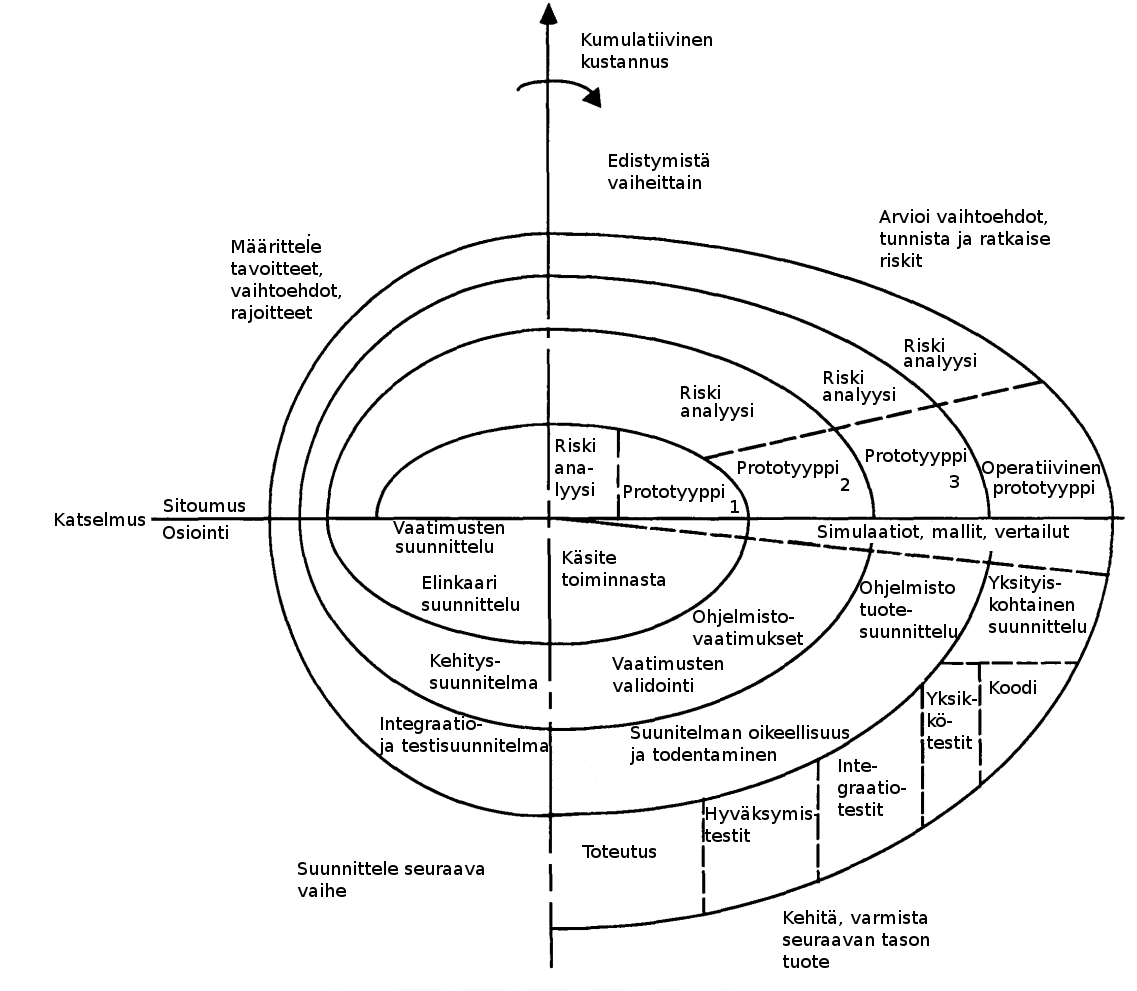
\includegraphics[width=\textwidth]{spiral}
\end{figure}

Spiraalimallissa jokainen vaihe aloitetaan tunnistamalla: \cite{BOE88}

\begin{itemize}
\item laadittavien ohjelmisto-osien suorituskykyyn, toiminnallisuuteen sekä sopeutumiskykyyn liittyvät tavoitteet
\item vaihtoehtoiset toteutustavat (ohjelmiston osto, ohjelmiston uudelleenkäyttö, vaihtoehtoiset ohjelmat)
\item ohjelmiston eri vaihtoehdoille asettamien rajoitteet (rajapinnat, aikataulu, kustannukset)
\end{itemize}

Seuraava askel on arvioida vaihtoehtoja suhteessa ohjelmiston tavoitteisiin ja rajoitteisiin. Usein tämä prosessi tunnistaa epävarmoja alueita, jotka ovat merkittäviä riskin lähteitä. Seuraava askel pitää sisällään kustannustehokkaan strategian muotoilun havaittujen riskien ratkaisemiseksi. Tähän voi liittyä prototyyppien valmistamista, simulointia, vertailuanalyysia, kyselylomakkeita, analyyttista mallinnusta, tai näiden yhdistelmiä sekä muita riskien ratkaisumenetelmiä \cite{BOE88}.

Jos suorituskykyyn tai käyttöliittymään liittyvät riskit hallitsevat ohjelman kehittämistä, seuraavassa vaiheessa määritellään ohjelmiston yleistä luonnetta, suunnitellaan seuraavan tason prototyyppiä ja kehitetään yksityiskohtaisempaa prototyyppiä riskien ratkaisemiseksi \cite{BOE88}.

Riskienhallinnan avulla aikaa ja työmäärää voidaan kohdentaa ongelma-alueisiin: toiminnan suunnitteluun (planning), asetuksien hallintaan (configuration management), laadun varmistukseen (quality assurance), muodolliseen todentamiseen (formal verification) tai testaukseen \cite{BOE88}.

Spiraalimallin tärkeä ominaisuus on, että jokainen iteraatio päätetään katselmukseen tuotteeseen liittyvän henkilöstön tai organisaation kanssa. Spiraalimallissa ei määritellä iteraatioiden pituutta suhteessa ohjelmistokehitykseen vaadittuun aikaan. Mallissa painotetaan vahvasti prototyypin osuutta ohjelmiston kehityskaaren aikana. Varhainen prototyyppi mahdollistaa ohjelmiston testattavaksi, jotta virheitä voidaan löytää aikaisessa vaiheessa \cite{BOE88}.

Spriraalimallin riskien analysoinnista huolimatta, ohjelmiston kehitysprosessi sisältää haasteita ohjelmiston vaatimusten hallintaan, laatuun ja erityisesti testaukseen liittyen. Spriraalimallissa ohjelmiston testausta tehdään prototyypin kehityskaaren lopussa ja palautetta asiakkaalta saadaan vasta iteraation lopussa. Spriraalimallissa ei ole korostettu vaatimuksien tärkeys\-järjestystä eikä hallinointia \cite{BOE88}.

Seuraavaksi tarkastelemme ketteriä kehitysmenetelmiä sekä miten nämä menetelmät ovat pyrkineet ratkaisemaan aikaisemmin käsiteltyjen suunnitelmavetoisten menetelmien puutteita ja miten ketterät menetelmät lähestyvät kappaleessa kaksi käsiteltyjä ohjelmistotuotannon haasteita ja ohjelmiston laatua.

Suunnitelmavetoisten prosessimallien ongelmien seurauksena useat ohjelmistoalan ihmiset ja organisaatiot kehittivät menetelmiä ja käytäntöjä, joille muutokset ovat hyväksyttyjä.
Menetelmiä kehitettiin useita ja eri maissa: \cite{WIC03}

\begin{itemize}
\item taipuisa järjestelmän kehitysmenetelmä (Dynamic Systems Development) Euroopassa
\item toiminnallisuusvetoinen kehitysmenetelmä (Feature-Driven Development) Australiassa
\item ja XP (Extreme Programming) \cite{BEC99}, Crystal \cite{COC05}, mukautuva ohjelmistokehitys (Adaptive Software Development) ja Scrum \cite{SCH09} Yhdysvalloissa.
\end{itemize}


Kaikilla ketterien menetelmien lähestymistavoilla oli tarkoitus välttää, lineaarista vaihe kerrallaan etenevää, suunnitelma- ja dokumenttivetoisuutta \cite{LAB03}.
Helmikuussa 2001 17 ketterien menetelmien kehittäjää tapasi keskustellakseen prosessimallien ja kokemuksiensa yhtäläisyyksistä  \cite{WIC03}.

Osallistujat määrittelivät käytännöt ketteriksi menetelmiksi ja kirjoittivat ''Manifesto for Agile Software Development''-julistuksen, mikä kuvaa ketterän kehityksen perusarvojaa \cite{WIC03}:

\begin{itemize}
\item yksilöt ja vuorovaikutus ennen prosesseja ja työkaluja
\item toimiva ohjelmisto ennen kattavaa dokumentaatiota
\item asiakasyhteistyö ennen sopimusneuvotteluja
\item muutoksiin vastaaminen ennen suunnitelman seuraamista.
\end{itemize}

Ohjelmistotuotannon parissa työskentelevät huomasivat, että ohjelmistoala erosi huomattavasti muista insinööritieteistä. Ohjelmiston valmistaminen on empiirinen prosessi, jonka lopputuloksena syntyy uusi tuote. Autojen kokoaminen on määriteltävä prosessi. Insinöörit voivat suunnitella prosessin, määritellä kokoonpanojärjestyksen sekä työntekijöiden, koneiden tai robottien toimenpiteet \cite{WIC03}.

Empiirinen prosessi vaatii \textit{tarkkaile ja mukaudu} (inspect and adapt) tyyppisen lähestymistavan. Oleellista oppia ja mukautua prosessin edetessä, eikä määritellä kaikkea alussa kattavasti.  Lyhyet iteraatiot mahdollistavat ketteriä menetelmiä mukautumaan ja muuttamaa liiketoimintaympäristön ennustamattomien vaatimuksien mukaan. Lyhyt kehityssyklin jälkeen ohjelmistokehityksen suuntaa voidaan tarvittaessa nopeasti muuttaa  \cite{WIC03}.

Kerromme seuraavaksi lyhyesti kahdesta ketterästä kehitysmenetelmästä. Selvitämme miten suunnittelua on lähestytty näissä menetelmissä ja miten niiden käytänteet ovat pyrkineet ratkaisemaan ohjelmistotuotannon haasteita ja laatuun liittyviä ongelmia. Käsittelemme näiden ketterien menetelmien ratkaisuja toisessa kappaleessa esitettyihin ohjelmistotuotannon haasteisiin. 

\subsection{Extreme programming}

XP (Extreme Programming) pienentää ohjelmistonkehityksen kustannuksia tekemällä jatkuvasti suunnittelua, määrittelyä, analysointia, ohjelmointia ja testausta ohjelmistokehityksen aikana.  \cite{BEC99}.

XP:ssä asiakas suunnittelee yhdessä kehittäjätiimin kanssa ohjelmiston toiminnallisuuksia, XP:ssä tarinoita (story), ja valitsee niistä eniten arvoa tuottavat toiminnallisuudet, jotka ovat arviotavissa ja testattavissa. Ohjelmoijat jakavat tarinat pieniksi käsiteltävän kokoisiksi ja ohjelmoitaviksi tehtäviksi (task). Ohjelmoijat suunnittelevat tehtävien pohjalta testejä, joiden avulla hän ymmärtää ohjelmistosta yhä enemmän. Nämä testit osoittavat läpäistessään tehtävän valmistuneen \cite{BEC99}.

XP:n testivetoinen ohjelmistokehitys (test-driven development, TDD) poikkeaa merkittävästi suunnitelmavetoisista menetelmistä, joissa vasta valmista ohjelmistoa tai prototyyppiä testataan. Testivetoisessa ohjelmakehityksessä uutta tuotantokoodia lisätään vasta, kun tuotantokoodille on olemassa yksi tai useampi testitapaus.

XP:n käytäntöihin kuuluu myös jatkuva pariohjelmointi (pair programming). Parin kanssa työskentelemällä ohjelmoijat ajavat testejä ja kehittävät samalla mahdollisimman yksinkertaista suunnitelmaa tehtävän ratkaisemiseksi \cite{BEC99}.

\subsection{Scrum}

Scrum on empiirinen, tarkkaileva ja mukautuva prosessi, jonka edetessä sitä pyritään parantamaan saatujen havaintojen perusteella. Scrum perustaa kaiken käytännön iteratiiviselle ja inkrementaaliselle prosessille: Jokaisen kehityssyklin tulos on valmiin ohjelmistotuotteen kehitys ja mahdollisesti julkaistavissa oleva ohjelmisto. \cite{SCH09}.

Scrum hallinnoi ohjelmistotuotannon monimutkaisuutta seuraavilla yksinkertaisilla käytänteillä: Iteraatioita kutsutaan sprinteiksi (sprint). Sprintti on 30 päivän iteraatio, jonka aika tuotetaan \textit{valmiin} (done) määritelmän mukainen ohjelmisto. Määritelmästä valmis sopii kehittäjätiimi, mitä sillä kyseessä olevassa projektissa tarkoitetaan. Usein se tarkoittaa, että toiminnallisuudet tulee olla kattavasti testattu ja ohjelmakoodi rakenteellisesti selkeää ohjelmakoodia (clean code) \cite{SCH09}. 

Sprintti aloitetaan sprintin suunnittelupalaverilla (sprint planning meeting), jossa valitaan kehitettävät toiminnallisuudet. Sprintin lopussa pidetään sprinttikatselmus (sprint review meeting), jossa ohjelmistoversio esitellään sidosryhmille \cite{SCH09}.

Scrumissa on kolme roolia: tuoteomistaja (Product owner), kehittäjätiimi (team) ja scrummaster (Scrum master). Tuoteomistaja on asiakasedustaja, joka rahoittaa ja visioi ohjelmistotuotteen. Kehittäjätiimi vastaa ohjelmiston toteuttamisesta ja scrummaster vastaa käytänteiden toteutumisesta ja opastaa kehittäjätiimiä saavuttamaan tavoitteensa \cite{SCH09}.

Scrum määrittelee neljä ohjelmistokehityksessä käytettävää tuotosta (artifact): tuotteen kehitysjono (product backlog), sprintin tehtävälista (sprint backlog), edistymiskäyrä (burndown chart) ja tuoteversio (increment of potentially shippable product functionality) \cite{SCH09}.

Asiakkaalta saadut ohjelmistojärjestelmän vaatimukset listataan tuotteen kehitysjonossa, jota käytetään suunnittelussa ja vaatimusten hallinnassa koko ohjelmistokehitysprosessin ajan. Tuoteomistaja on vastuussa tuotteen kehitysjonon sisällöstä ja vaatimusten tärkeysjärjestyksestä \cite{SCH09}.

Sprintin tehtävälista sisältää tehtävät, jotka kehittäjätiimi toteuttaa  julkaistavaksi tuotteen toiminnallisuudeksi. Sprintin tehtävälista on läpinäkyvä reaaliaikainen kuvaus työstä, jonka kehittäjätiimi suunnittelee saavansa valmiiksi sprintin aikana. Tehtävälista pitää sisällään kunkin tehtävän kuvauksen, vastuullisen toteuttajan, tehtävän tilanteen (ei aloitettu, kesken, valmis), sekä jäljellä oleva arvioitu aika työtunteina. \cite{SCH09}.

Edistymiskäyrä ilmaisee visuaalisesti jäljellä olevan työmäärän ja ajan suhdetta. Edistymiskäyrällä voidaan peilata todellista työn edistymistä ja nopeutta projektin suunnitelmiin ja toiveisiin \cite{SCH09}.

Scrum vaatii kehitystiimiä rakentamaan uuden tuoteversion jokaisessa sprintissä. Tuoteversio on toimiva ohjelmisto, johon jokaisessa iteraatiossa on lisätty uusia täysin testattuja toiminnallisuuksia \cite{SCH09}.

\section{Ketterien menetelmien ratkaisuja}

Seuraavaksi tarkastelemme, mitä kappaleessa 3.3 ja 3.4 käsiteltyjen ketterien menetelmien käytänteet tarjoavat ratkaisuna kappaleessa kaksi esitettyihin ohjelmistotuotannon haasteisiin ja laadunhallintaan.

XP:n käytäntöihin kuuluu jatkuva pariohjelmointi ja testivetoisuus. Nämä käytänteet poikkeavat muista kappaleessa kolme esitettyjen menetelmien käytänteistä, joten käsittelemme tarkemmin testivetoisuutta kappaleessa 4.4 sekä pariohjelmointia kappaleessa 4.5. Tarkastelemme erityisesti niiden vaikutusta ohjelmiston laatuun.  

\subsection{Koordinointi ketterissä menetelmissä}

Toisessa kappaleessa totesimme ohjelmistotuotannon haasteiden liittyvän koordinointiin, ja ongelman osa-alueiden olevan muuttuvien vaatimuksien lisäksi henkilöstön hallinta sekä ajallisten ja taloudellisten resurssien käyttö. 

Ketterät menetelmät lähestyvät henkilöstöhallintaa suunnitelmavetoisia menetelmiä joustavammin ja ihmisläheisemmin: kehittäjätiimit ovat usein itseorganisoituvia ja he tekevät tekniset ratkaisut itse. Ketterät menetelmät hylkäävät ajatuksen, että ihmiset olisivat vaihdettavissa olevia osia. Yksilöiden ajatellaan olevan päteviä ammattilaisia, jotka osaavat suunnitella työnsä ja tietävät keinot saavuttaa paras tulos \cite{FOW01a}.

Ketterissä menetelmissä kehittäjien on kyettävä tekemään kaikki tekniset ratkaisut \cite{FOW01a}. XP:ssä suunnitteluprosessin (planning game) aikana tiimi arvio omien kokemuksiensa perusteella toiminnallisuuksien kehittämiseen vaadittavan ajan \cite{BEC99}.

Scrumissa kaikki projektin hallinnolliset vastuut on jaettu kolmen, kappaleessa 3.4 mainittujen, roolien kesken. Tuoteomistajan vastuu on esitellä kehittäjätiimille ja muille projektiin osallistuville tuotteelle asetettavat vaatimukset. Tuoteomistaja laatii alustavan vaatimusmäärittelyn, sijoitettavalle pääomalle asetettavat tavoitteet (ROI) ja julkaisusuunnitelmat (relese plans) \cite{SCH09}.

Kehittäjätiimin vastuulla on toiminnallisuuksien kehittäminen. Ohjelmoijat päättävät, miten uusi toiminnallisuus toteutetaan ja työskentelevät rauhassan lopun iteraation ajan. Kehitystiimi on eri alojen asiantuntemuksesta koostuva itseorganisoituva ryhmä. Kehitystiimi on yhdessä vastuussa jokaisen iteraation onnistumisesta \cite{SCH09}.

Kehittäjätiimi kokoontuu kokoontuu joka päivä 15 minuutin tapaamiseen - päiväpalaveriin (Daily Scrum). Jokainen tiimin jäsen vastaa kolmeen kysymykseen: Mitä olen tehnyt viimeisen tapaamisen jälkeen? Mitä ajattelin tehdä seuraavaksi? Mikä estää minua saavuttamasta tavoitteitani? Tapaamisen tarkoituksena on koordinoida tiimin työtä päivittäin ja sopia tarvittavista tapaamisista \cite{SCH09}.

Scrummaster on vastuussa scrumprosessista. Hänen tehtävänä on esitellä scrumin periaatteet jokaiselle projektiin osallistuvalle. Scrummaster vastaa, että scrum sopii organisaation kulttuuriin ja toteuttaa odotetut hyödyt. Scrummaster valvoo, että jokainen toteuttaa scrumin käytänteitä: Tuoteomistaja hallinnoi ja priorisoi ohjelmiston toiminnallisuuksia tuotteen kehitysjonon kautta. Kehittäjätiimin tulee pitää päiväpalaverit sekä ylläpitää sprintin tehtävälistaa ja edistymiskäyrää. Kehittäjätiimille on taattava työrauha eikä tehtävälistan toiminnallisuudet ja niiden tärkeysjärjestys saa muuttua kesken meneneillä olevaa sprinttiä \cite{SCH09}.

Ketterissä menetelmissä asiakas on läheisessä yhteistyössä koko ohjelmistotuotantoprosessin ajan. Jokaisessa iteraatiossa asiakas voi tarkistaa kehityksen vaihetta ja muuttaa sen suuntaa. XP:ssä asiakas on jatkuvasti paikalla (on-site customer). Jos kehittäjätiimille ilmenee kysymyksiä toteutuksesta tai toiminnallisuuden laajuudesta, ohjelmoijat voivat keskustella asiakkaan kanssa \cite{BEC99}. Tämä johtaa läheisempään asiakassuhteeseen ohjelmiston kehittäjien kanssa. Läheinen asiakassuhde on edellytys mukautuvan prosessin onnistumiselle \cite{FOW01a}.

Scrumissa sprinttikatselmuksesssa tiimi esittelee tuoteomistajalle ja muille halukkaille sidosryhmille, iteraation aikana, kehitetyt toiminnallisuudet. Tapaamisen tarkoituksena on tuoda ihmiset yhteen, esitellä ohjelmiston toiminnallisuudet ja auttaa osallistujia yhdessä päättämään projektin seuraavasta iteraatiosta \cite{SCH09}.

Sprinttikatselmuksen jälkeen scrummaster ja tiimi pitää sprintin retrospektiivin (Sprint retrospective meeting). Kehittäjätiimi käy läpi sprintin aikaisen prosessin heikkouksia ja vahvuuksia, kehittääkseen sitä edelleen parempaan suuntaan seuraavaan iteraatioon \cite{SCH09}.


\subsection{Suunnittelu ketterissä menetelmissä ja muuttuvat vaatimukset}

Suunnitelmavetoisissa menetelmissä suunnittelutyöhön kuluu kaavioita, joilla voidaan kuvailla ohjelmiston rakennetta ja käyttäytymistä. Ketterien menetelmien prosesseissa suunnittelussa painotetaan joustavuutta, jotta suunnitelmaa voidaan helposti muuttaa kun vaatimukset muuttuvat \cite{FOW01b}.

XP:ssä suunnitelmien ja kaavioiden merkitys on vähäinen: kaavioita tulee käyttää, jos niistä on hyötyä. Äärimäiset XP:n toteuttajat eivät käytä kaavioita lainkaan \cite{FOW01b}.

XP:n näkökulmasta kaavioiden tarkoitus on tarjota yhteydenpitoa. Tehokkaan yhteydenpidon takaamiseksi on piirrettävään kaavioon valittava tärkeät asiat ja vältettävä vähemmän tärkeitä. Vain merkitykselliset luokat sekä niiden tärkeimmät attribuutit ja operaatiot kuvataan kaavioon \cite{FOW01b}.
Ohjelmoinnin aikaista dokumentointia voidaan muuttuviin vaatimuksiin ja suunnitelmiin sopeuttaa seuraavasti: \cite{FOW01b}

\begin{itemize}
\item Käytetään vain kaavioita, joita voidaan pitää ajan tasalla helposti
\item Laitetaan kaaviot paikkaan, jossa ne ovat helposti nähtävillä
\item Kannustetaan ihmisiä muuttamaan kaavioita
\item Heitetään pois kaaviot, joita ihmiset eivät käytä.
\end{itemize}

Usein kaavioita käytetään välittämään tietoa eri ryhmien välillä. XP:tä toteuttaville kaaviot ovat toiminnallisuuksia muiden joukossa, joiden arvon määrää asiakas. Kaaviot ovat hyödyllisiä vain jos ne auttavat viestinnässä. Ohjelmakoodin varasto (repository) on yksityiskohtaisen tiedon lähde ja kaaviot koostavat ja korostavat tärkeitä asioita \cite{FOW01b}.

Ketterissä menetelmissä suunnittelua tehdään koko ohjelmistokehityskaaren aikana: jos ohjelmistokoodi on vaikea muuttaa, ei projektin aikana tehdä riittävästi rakenteeseen liittyvää suunnittelua. Ohjelmistokehityksen aikana ohjelmakoodi on pidettävä yksinkertaisena ja selkeänä \cite{FOW01b}.
Ohjelmakoodin rakennetta on tarpeen vaatiessa jatkuvasti parannettava rakennemuutoksilla (refactoring). Ohjelmoijien on ymmärrettävä suunnittelumallien (design patterns) tarjoamat ratkaisut sekä osattava käyttää niitä. Suunnittelumallit ovat hyväksi havaittuja ratkaisuja ohjelmistokehityksessä usein esiityviin suunnitteluongelmiin \cite{FOW01b}.

Ohjelmistoa on suunniteltava ottaen huomioon, että ohjelmakoodia tullaan myöhemmin muuttamaan. Ohjelmiston rakenteesta on osattava viestiä, ohjelmakoodin, kaavioiden ja ennen kaikkea keskustelun avulla \cite{FOW01b}.

\subsection{Ketterät menetelmät ja ohjelmistojen laatu}

Koska muodollinen suunnittelu dokumentaation muodossa on vähäistä ja suunnitelmia heitetään pois \cite{FOW01b}, on aiheellista käsitellä, miten ohjelmiston laatu otetaan huomioon ketterien menetelmien ohjelmistosuunnittelussa.

Kolmannessa kappaleessa määrittelimme laadun kansainvälisen standarointiorganisaation laatupiirteiden mukaisesti. Niistä toiminnallisuus, luotettavuus, käytettävyys ja tehokkuus yhdistyy asiakkaan toiveisiin ja näkemykseen tuotettavasta ohjelmisto\-järjestelmästä \cite{KIP96}. Laatupiirteet liittyvät vaatimusten hallintaan, joka on tärkeä osa sekä XP:tä \cite{BEC99} että scrumia \cite{SCH09}. Toimiva ja testattu ohjelmisto on asiakkaan nähtävissä koko kehityskaaren ajan, joten asiakas näkee täyttääkö ohjelmisto hänen tarpeensa \cite{BEC99}.

Scrumissa tuoteomistajan näkemys tarvittavista toiminnallisuuksista on listattu tuotteen kehitysjonossa. Tuotteen kehitysjono on asiakkaan priorisoima: toiminnallisuudet jotka tuottavat arvoa ovat ylimpänä listassa. Muutokset tuotteen kehitysjonossa heijastavat muuttuvaa liiketoimintaympäristöä ja asiakas itse voi priorisoimalla vaikuttaa ohjelmiston vaatimuksiin sekä laatuun nähdessään siinä puutteita \cite{SCH09}.

XP:ssä asiakaan laatimat toiminnalliset testit (functional test) osoittavat, että toiminnallisuudet ovat asiakkaan näkemyksen mukaisia. Toiminnalliset testit ovat asiakkaan määrittämiä ohjelman käyttöön liittyviä testejä, joilla hän vakuuttuu toiminnallisuuden oikeanlaisesta toteutuksesta \cite{BEC99}.

Ketterissä menetelmissä on minimaalinen toimiva ohjelmisto valmis ensimmäisen iteraation jälkeen, sillä jokainen toteutettava toiminnallisuus tehdään valmiiksi. Asiakkaan käyttäessä toimivaa ohjelmisto\-järjestelmää, hän näkee mahdolliset puutteet toiminnallisuudessa ja käyttö\-liittymän käy\-tettävyydessä. Puutteet voidaan korjata seuraavassa iteraatiossa \cite{BEC99}.

Ketterät menetelmät ottavat huomioon laadunvarmistuksen asiakkaan vaatimusten osalta. Kansainvälisen standardointiorganisaation laatupiirteet ylläpidettävyys ja siirrettävyys liittyvät myös ohjelmakoodin sisäiseen rakenteeseen ja laatuun (design quality) \cite{KIP96}.

Asiakkaalle ohjelmakoodin sisäisen laadun havaitseminen on vaikeampaa. Sisäinen laatu on asiakkaalle yhtä tärkeää kuin kehitystiimille, koska huonosti suunniteltua ohjelmistoa on kallista muuttaa. Asiakkaan tulee kuunnella kehitystiimi, ja jos he valittavat vaikeuksista tehdä muutoksia, on heille annettava aikaa korjata tilanne \cite{FOW01b}.

Tarkkailemalla poistettavan ohjelmakoodin määrää, voidaan nähdä tapahtuuko tarpeeksi suunnittelua. Ohjelmistoprojektissa, jossa tehdään riittävästi muutoksia rakenteeseen (refactoring), poistetaan tasaisesti huonoa ohjelmakoodia \cite{FOW01b}.

XP:ssä painotetaan yksinkertaista suunnitelmaa ja rakenteen jatkuvaa parantamista. Ohjelmoijat pyrkivät mahdollisimman selkeään ohjelmakoodiin. Jos ohjelmoijat näkevät toiminnallisuudelle paremman ratkaisun hyväksytysti ajettujen testien jälkeen, heidän tulee korjata ohjelmiston rakennetta \cite{BEC99}.
Scrumissa kehittäjätiimin määrittelee, milloin toteutettu toiminnallisuus on \textit{valmis}. Määritelmän mukaan toteutettu toiminnallisuus on oltava hyvin suunniteltu (well-structured) ja rakennettu (well-written code) ohjelmakoodi\cite{SCH09}.


\subsection{Ohjelmistojen testaus}

Testaus on XP:n ydinkäytäntöjä: kehittäjätiimin kaikki ohjelmoijat kirjoittavat testitapauksia. Ohjelmoijat varmistavat osaltaan ohjelmakoodin toimivuuden eikä ohjelmakoodia siirretä erilliselle testauksesta vastaavaalle organisaatiolle tai jäsenelle.

XP.ssä testejä tehdään aina ennen varsinaista tuotantokoodia: ohjelmoija kirjoittaa ensin testitapauksen, ja sen jälkeen tarvittavan määrän tuotantokoodia testitapauksen ratkaisemiseksi. Ohjelmistossa läsnäolevat ja ohjelmakoodin kattavat testit varmistavat jatkuvan integraation (continuos integration) ja vaakaan rakennusprosessin \cite{FOW01a}. Integroidessa uutta ohjelmakoodia ohjelmistoon, kaikki aikaisemmin tehdyt ja uudet testit ovat läpäistävä. Hyväksytysti ajettujen testien jälkeen voidaan muutokset hyväksyä ja uusi versio julkaista \cite{BEC99}.

Asiakas laatii kehittäjätiimin avulla hyväksymätestit (acceptance test), joiden avulla hän vakuutuu osaltaan uuden tarinan onnistuneesta toteutuksesta: Hyväksymätesti kattaa toiminnallisuuden testauksen koko ohjelmistojärjestelmätasolla kaikkiin tarvittaviin ohjelmisto-osiin käyttöliittymästä tietokantaan.

Hyväksymätestit käyttävät järjestelmää ohjelmallisesti käyttäjän tavoin: painavat käyttöliittymän painikkeita tai syöttävät tekstikenttiin tietoa sekä lukevat käyttäjälle näytettävää tulostetta. Oikeat syötteet ja tulosteet kertovat järjestelmän toiminnasta sekä takaavat ohjelmoijille ja sidosryhmille, että ohjelmisto toimii vaatimusten mukaisesti. Testit ovat ajettavissa koko ohjelmiston kehityskaaren ajan ja ne takaavat ohjelmiston toimivuuden jatkuvasti. Toiminnallisuuksia lisättäessä tai ohjelmakoodin rakennetta muutettaessa testit kertovat onko uusi versio toimiva järjestelmä \cite{BEC99}.

Scrumissa on kaikilla projektiin osallistuvien on yhteisesti sovittava määritel\-mästä \textit{valmis} toiminnallisuus. Valmiin määritelmän on vastattava organisaation standardeja, käytäntöjä ja ohjeita. Kun sprinttikatselmuksessa esitetään valmis toiminnallisuus, sen on oltava tämän sovitun määritelmän mukainen. Tuoteomistaja voi vaatia, että toiminnallisuuden valmistuessa se on oltava julkaistavissa. Toiminnallisuuden ohjelmakoodin täytyy olla tällöin hyvin rakennettu (well-structured code) ja kattavasti testattu \cite{SCH09}.

Winston Royce kirjoitti artikkelissaan ''Managing the development of large software systems'', että ohjelmoijan ei tule testata kirjoittamaansa ohjelmakoodia. Royce arvioi, että useimmat virheet ovat ilmiselviä ja ovat löydettävissä katsomalla ohjelmakoodia \cite{ROY70}. XP:ssä tämä on hyväksytty tosiasia ja ongelmaa on lähestytty työskentelemällä jatkuvasti pareittain, jolloin ohjelmoijat testaavat ja arvioivat toistensa ohjelmakoodia \cite{BEC99}.


XP:n testivetoisessa menetelmässä testitapaukset määrittävät ohjelmiston haluttua käyttäytymistä ja osoittavat oikein toteutetut toiminnallisuudet. Testivetoisessa kehityksessä toiminnallisuutta lisätään inkrementaalisesti ja valmiiksi toteutetut sekä vielä keskeneräiset toiminnallisuudet ovat tiimille selvillä koko kehitysprosessin ajan \cite{EDW03}.

Testivetoinen menetelmä eroaa merkittävästi suunnitelmavetoisista menetel\-mistä, joissa ohjelmiston testaus tapahtuu vasta ohjelmistokehityskaaren lopussa. Tästä johtuen on tarpeen tarkastella tarjoaako testivetoinen ohjelmistokehitys ratkaisuja ohjelmistotuotannon haasteisiin ja parantaako testivetoisuus ohjelmiston laatua. Käsittelemme seuraavaksi löytämiämme tutkimuksia ja niiden tuloksia testivetoisuuden hyödyistä.

Tietojen\-käsittely\-tieteen opiskelijoille tehdyssä tutkimuksessa opiskelijat kävivät vuonna 2003 ohjelmointikurssin noudattaen testivetoista menetelmää. Vertailuryhmänä käytettiin samaa kurssia vuodelta 2001, jolloin opiskelijat eivät käyttäneet testivetoista menetelmää. Tulokset osoittivat, että testivetoista menetelmää käyttäneillä opiskelijoilla oli keskimäärin 45\% vähemmän virheitä \cite{EDW03}.

IBM kokeili eräässä ohjelmistokehitysryhmässä testivetoista kehitys\-menetelmää, kun aikaisemmat laadunvarmistukset eivät tuottaneet toivottua tulosta. Käyttä\-mällä testivetoista menetelmää virheet vähenivät noin 50\% aikaisempaan verrattuna \cite{MAW03}.

Toisessa tutkimuksessa 24 ohjelmistoalan ammattilaista jaettiin kahteen ryhmään pareittain toimiviksi tiimeiksi. Toinen ryhmistä teki ohjelmistokehitystä testivetoisesti ja toinen ohjelmoi vesiputousmallin mukaisesti. Testivetoisesti ohjelmaa kehittäneet parit tuottivat laadukkaampaa ohjelmakoodia. Testivetoisen ryhmän ohjelmakoodi läpäisi 18\% enemmän testitapauksia kuin kontrolliryhmän ohjelmakoodi \cite{GEW03}.

Yllä mainitut tutkimukset osoittavat, että testivetoinen ohjelmistokehitys parantaa ohjelmiston laatua kun tarkastellaan ohjelmistossa esiintyviä virheiden määrää ja koodikattavuutta (code coverage). Koodikattavuus kertoo, kuinka paljon tehdystä tuotantokoodista on testattu. Tehdyissä kyselyissä testivetoisissa ryhmissä osallistuneet olivat luottavaisempia tekemistään ratkaisuista \cite{GEW03}.

\subsection{Pariohjelmointi}

Pariohjelmointi on toinen käytäntö, mikä erottaa XP:n muista ohjelmistotuotannon menetelmistä. Pariohjelmoinnin vaikutuksia haasteisiin ja laatuun on syytä tarkastella lähemmin. Kappaleessa 2.1 toimme haasteista esille muun muassa henkilöstön hallinnan, aikataulun ja taloudellisten resurssien käytön. Kappaleessa 2.4 käsittelimme ohjelmiston laatua. Tarkastelemme seuraavaksi pariohjelmoinnista löytämiämme tutkimuksia ja niiden tuloksia erityisesti laatuun sekä hieman myös kustannuksiin liittyen.

Pariohjelmoinnissa kaksi ohjelmoijaa yhdessä työstävät yhtä ohjelmakoodia, algoritmia tai suunnitelmaa. Toinen parista ohjelmoi ja toinen heistä tarkkailee etsien virheitä, miettien vaihtoehtoja, tutkien lähteitä ja miettien erilaisia toteutustapoja. Parit vaihtavat roolejaan ajoittain. Molemmat ovat tasavertaisia ja aktiivisia osallistujia \cite{WIL00}.

Vuonna 1998 John Nosek teki tutkimuksen, jossa kokeneet ohjelmoijat työskentelivät haastavien, omalle organisaatiolleen tärkeiden, tehtävien parissa omassa työskentely-ympäristössään. Kukaan osallistujista ei ollut työskennellyt annetun tehtävän kaltaisen ongelman parissa aikaisemmin. Annetun tehtävän kaltaista ongelmaa pidettiin organisaatiolle menestykselle tärkeänä ja niin vaativana, että yleensä tehtäviin palkattiin ulkopuolisia konsultteja \cite{NOS98}.

Koehenkilöt valittiin satunnaisesti työskentelemään pareittain testiryhmään ja yksilöinä kontrolliryhmään.
Ryhmiltä tehtäviin kulunut aika mitattiin. Ratkaisuista pisteytettiin luettavuus väliltä 0-2. Lukuarvo 0 tarkoitti lukukelvotonta ratkaisua ja 2 täysin luettavissa olevaa ratkaisua. Ratkaisun toimivuus pisteytettiin väliltä 0-6. Lukuarvo 0 merkitsi, että ratkaisu ei saavuttanut annettua tehtävää lainkaan. Täysin toimiva ratkaisu pisteytettiin arvolla 6. Kokonaispistemäärän maksimiarvo oli 8, joka oli luettavuuden ja toimivuuden summa \cite{NOS98}.

Pareittain työskentelevät saivat keskimäärin kokonaispistemääräksi 7,6 ja aikaa kului 30,2 minuuttia. Vertailuryhmän keskimääräinen kokonaispistemäärä oli 5,6 ja tehtävään aikaa kului 42,6 minuuttia \cite{NOS98}.

Vuonna 1999 Utahin yliopiston tietojenkäsittelytieteen opiskelijat osallistuivat tutkimukseen. Opiskelijat jaettiin kahteen ryhmään. Kolmetoista opiskelijaa muodosti kontrolliryhmän, jossa opiskelijat työskentelivät itsenäisesti kaikissa annetuissa tehtävissä. 28 opiskelijaa muodosti testiryhmän, jossa opiskelijat muodostivat kahden hengen ryhmän. Kokeilu vertaili tehtävistä suoriutumiseen vaadittua aikaa, tuottavuutta ja suoritettujen tehtävien laatua ryhmien välillä. Ohjelmille suoritettiin automaattiset testit ohjelmointityön laadun arvioimiseksi. Taulukossa 1 on tutkimustulos Utahin opiskelijoille tehdystä pariohjelmoinnista \cite{WIL00}:
Taulukko 1. Läpäistyt testitapaukset prosentteina
\begin{center}
\begin{tabular}{ | l | l | p{5cm} |}
\hline
Tehtävä & Yksin työskentelevät & Pareittain työskentelevät \\ \hline
Ohjelma 1 & 73,4 & 86,4 \\ \hline
Ohjelma 2 & 78,1 & 88,6 \\ \hline
Ohjelma 3 & 70,4 & 87,1 \\ \hline
Ohjelma 4 & 78,1 & 94,4 \\ \hline
\end{tabular}
\end{center}

Monet opiskelijat olivat epäluuloisia pariohjelmoinnin hyödyistä: he pohtivat paljonko ylimääräistä kommunikaatiota vaaditaan, miten he sopeutuvat toistensa työskentelytapoihin, ohjelmointityyliin ja miten heidän egonsa vaikuttavat työskentelyyn, sekä miten erimielisiä he ovat tehtävien toteutuksista. Tosiasiassa ohjelmoijat käyvät läpi siirtymäajan yksinäisestä työskentelystä yhteisölliseen työskentelytapaan. Siirtymäajan kuluessa he oppivat sopeuttamaan toimintojaan käyttämään hyväksi vahvuuksiaan ja välttämään heikkouksia. Tuloksena ryhmän tuottavuus ylittää ryhmän yksilöiden tuottavuuden summan \cite{WIL00}.

Nosekin tekemässä tutkimuksessa pareittain työskentelevät käyttivät, työskennellessään rinnakkain, yhteensä 60\% enemmän ohjelmointiaikaa kuin yksin työskentelevät \cite{NOS98}. Utahin opiskelijoille tehdyssä tutkimuksessa saatiin samankaltaisia tuloksia: keskimäärin pareittain työskenteleviltä vaati yhteensä 60\% enemmän ohjelmointiaikaa annetusta tehtävästä suoriutumiseen \cite{WIL00}.

Siirtymäajan jälkeen pareittain työskentelevät opiskelijat paransivat tuloksiaan. Pareittain työskenteleviltä vaadittu ohjelmointiaika oli enää 15\% suurempi kuin yksin työskentelevillä. Tässä vaiheessa opiskelijat olivat tottuneet pariohjelmointiin ja toistensa työskentelytapoihin \cite{WIL00}.

Laurie Williamsin, Ward Cunninghamin ja Ron Jeffriesin haastattelemat ohjelmoijat sanoivat, että pareittain analysointi ja suunnittelu on tärkeämpää kuin toiminnallisuuden toteuttaminen. Ohjelmoijat usein toteuttavat yksilöllisesti rutiinitehtäviä ja yksinkertaisia ohjelmakoodeja. Tällaisten tehtävien toteuttaminen yksilöllisesti tehtynä tehokkaampaa \cite{WIL00}.

Pareittain työskentelevät tuottavat luettavampaa ohjelmakoodia ja toimivampia ratkaisuja kuin yksin toimivat ohjelmoijat. Ryhmissä toimivat ratkaisevat ongelmia keskimäärin nopeammin kuin yksilöt. Lisäksi pareittain toimivat ilmaisevat korkeampaa luottamusta ratkaisuunsa ja kokevat nauttivansa prosessista enemmän kuin yksilöinä ohjelmoivat \cite{NOS98}.

Pareittain ohjelmoivat ihmiset tekevät erityisesti parempaa suunnittelua ja analyysia kuin yksilölliset ohjelmoijat. Pari harkitsee huomattavasti enemmän vaihtoehtoja ja yhtyvät nopeasti toteutettavaan ratkaisuun. Ideoiden vaihto parin välillä vähentää huonon suunnitelman todennäköisyyttä. Yhdessä työskentelemällä pari voi toteuttaa tehtäviä, jotka voivat olla liian haastavia yhdelle. Parityöskentely pakottaa osallistujia keskittymään täysin haasteena olevaan tehtävään \cite{WIL00}.

Pariohjelmoinnin kustannukset ovat oleellinen asia. Voisi olettaa, että pariohjelmoinnin sisällyttäminen ohjelmistotuotantoon kaksinkertaistaa kustannukset jos henkilöstömäärää on lisättävä samassa suhteessa. John Nosekin \cite{NOS98} sekä Williamsin, Kesslerin, Cunninghamin ja Jeffriesin \cite{WIL00} aiheesta tekemät tutkimukset osoittavat, että pareittain työskentelevät tiimit suoriutuvat tehokkaammin kuin yksittäiset ohjelmoijat. Tämä huomioden kustannukset eivät nouse suoraan verrannollisesti henkilöstömäärän kanssa. Laadunvarmistuksesta aiheutuvat kustannukset huomioiden pareittain ohjelmointi saattaa olla kustannustehokkaampaa kuin yksilöllisesti ohjelmoitaessa \cite{COC00a}.

\section{Yhteenveto}

Tässä tutkielmassa kävimme läpi ohjelmistotuotannon haasteita ja ohjelmiston laatuun liittyviä määritelmiä. Selvitimme miten suunnitelmavetoiset ja ketterät menetelmät ovat lähestyneet ohjelmistotuotantoa. Tarkastelimme mitä ketterät menetelmät ovat tarjonneet ratkaisuna haasteille sekä miten laadunhallinta otetaan huomioon ketterissä menetelmissä, ja onko ketterien menetelmien käytänteillä ollut vaikutusta ohjelmistojen laatuun. 

Ketterien menetelmien käytänteistä ja vaikutuksesta laatuun käsittelimme testivetoisuutta ja pariohjelmointia. Totesimme, että pariohjelmointi on usein jopa kustannustehokkaampaa kuin yksin ohjelmoitaessa, jos huomioidaan laadunvarmistuksen kustannukset. Pariohjelmointi tuottaa paremmin suunniteltua ohjelmakoodia ja parempia ratkaisuja kuin yksin ohjelmoitaessa. 

Testivetoisuuden totesimme tuottavan laadukkaampaa ohjelmakoodia kuin vesiputousmallin mukaisesti ohjelmoitaessa. Testivetoisesti ohjelmoineet ovat luottavaisempia omaan ratkaisuunsa. 

Ohjelmistojen kehittäminen internet-aikakaudella vaatii joustavia kehitysmenetelmiä, jotka sopeutuvat nopeasti vaihtuviin vaatimuksiin ja vaativiin markkinoihin. Ketterät menetelmät sopeutuvat perinteisiä menetelmiä paremmin tällaisiin ympäristöön.

Suunnitelmavetoisissa menetelmissä ajatuksena on, että riittävällä työllä voidaan ennakoida vaatimukset täydellisesti sekä alentaa ohjelmistotuotantoon liittyviä kustannuksia vähentämällä muutoksia. Ketterät menetelmät pyrkivät alentamaan uudistusten kustannuksia \cite{WIC03}. Ketterät menetelmät ovat valmiimpia muutoksille. Liiketoimintaympäristö vaatii sekä odottaa innovatiivisia, korkealuokkaisia ohjelmistoja, jotka vastaavat niiltä odotettuihin vaatimuksiin \cite{BRL03}.

Ketterät menetelmät tarjoavat vaatimusten hallinnalla ja kevyillä organisatorisilla rakenteilla ratkaisuja ohjelmistotuotannon haasteisiin ja ohjelmiston laadunhallintaan. Onnistunut ohjelmistokehityksen aikainen rakenteen suunnittelu parantaa ohjelmiston sisäistä laatua. XP:n jatkuva testaus antaa mahdollisuuden toteuttaa rakennemuutoksia toiminnallisuuksia rikkomatta. Testivetoisella ohjelmistokehityksellä voidaan parantaa sekä ohjelmiston sisäistä että käyttäjän kokemaa laatua. Pariohjelmoinnilla ohjelmiston suunnittelu ja laatu tehostuu merkittävästi.



% --- Back matter ---
%
% bibtex is used to generate the bibliography. The babplain style
% will generate numeric references (e.g. [1]) appropriate for theoretical
% computer science. If you need alphanumeric references (e.g [Tur90]), use
%
% \bibliographystyle{babalpha}
%
% instead.

\bibliographystyle{babplain}
\bibliography{references-fi}


\end{document}
